%This is an example for a chapter, additional chapter can be added in the skeleton-thesis
%To generate the final document run latex, build and quick build commands on the skeleton-thesis file not this one.
\chapter{Introduction}
Android is by far the most popular smartphone operating system at the time of this writing. With around 75\% of the global smartphone market~\cite{Perez}, its application ecosystem has grown along with it.  According to a recent Google press release, Google Play now has around 700,000 applications~\cite{Womack}. Unlike the Apple iOS ecosystem whose applications are centrally verified before becoming available, Android applications are more lightly vetted. This puts more responsibility on the user to make the important decision of which applications they trust. The permissions architecture employed by Android, however, makes these trust decisions more difficult. 

\subsection{Mobile Device Permission Models}
In the current implementation, application developers are responsible for defining the set of permissions their application asks for independent of what their application’s code actually uses~\cite{Felt}. The list is presented to the user at install-time whether installing an 
application obtained through the Google Play market or elsewhere. This list contains the canonical names given to each permission object, but provides little context as to what the permission is being used for. In the latest API, Google has added more description and added warning levels . At the end of the day, however, users have no choice but to accept the permissions list as presented to them, or not install the application.

While all smartphone applications are susceptible to being over permissioned, Apple's iOS and Blackberry's OS both give the user the ability to revoke an applications permissions. iOS uses a "dynamic" permissions model; the user is prompted once per application to use phone features such as the GPS receiver. The user then has the option of changing their decision through the system's settings menu. 

Blackberry OS uses a "static" approach similar to that of Android. Application developers declare the set of permissions they would like their program to have, and this list is presented to the user at installation. However, unlike Android, the user has the option to edit the list and revoke any permission. This approach adds a degree of granularity to an otherwise binary trust decision and is the approach explored in this study.

\subsection{Removing Permissions from Android Apps}

Shown in Figure~\ref{fig:permission}, is the application permissions listing for a Flashlight application obtained through the Play market.  While one could reason this application would only need the hardware controls necessary to turn on the phone's light, due to the large quantities of ad network libraries and other debris embedded within, it asks for much more. If permissions were editable, the user would be able to trust this application’s ability to operate the flashlight only, and not have to worry about the true reason for the other permission requests.

\begin{figure}[t]
\centerline{\resizebox{0.4\linewidth}{!}{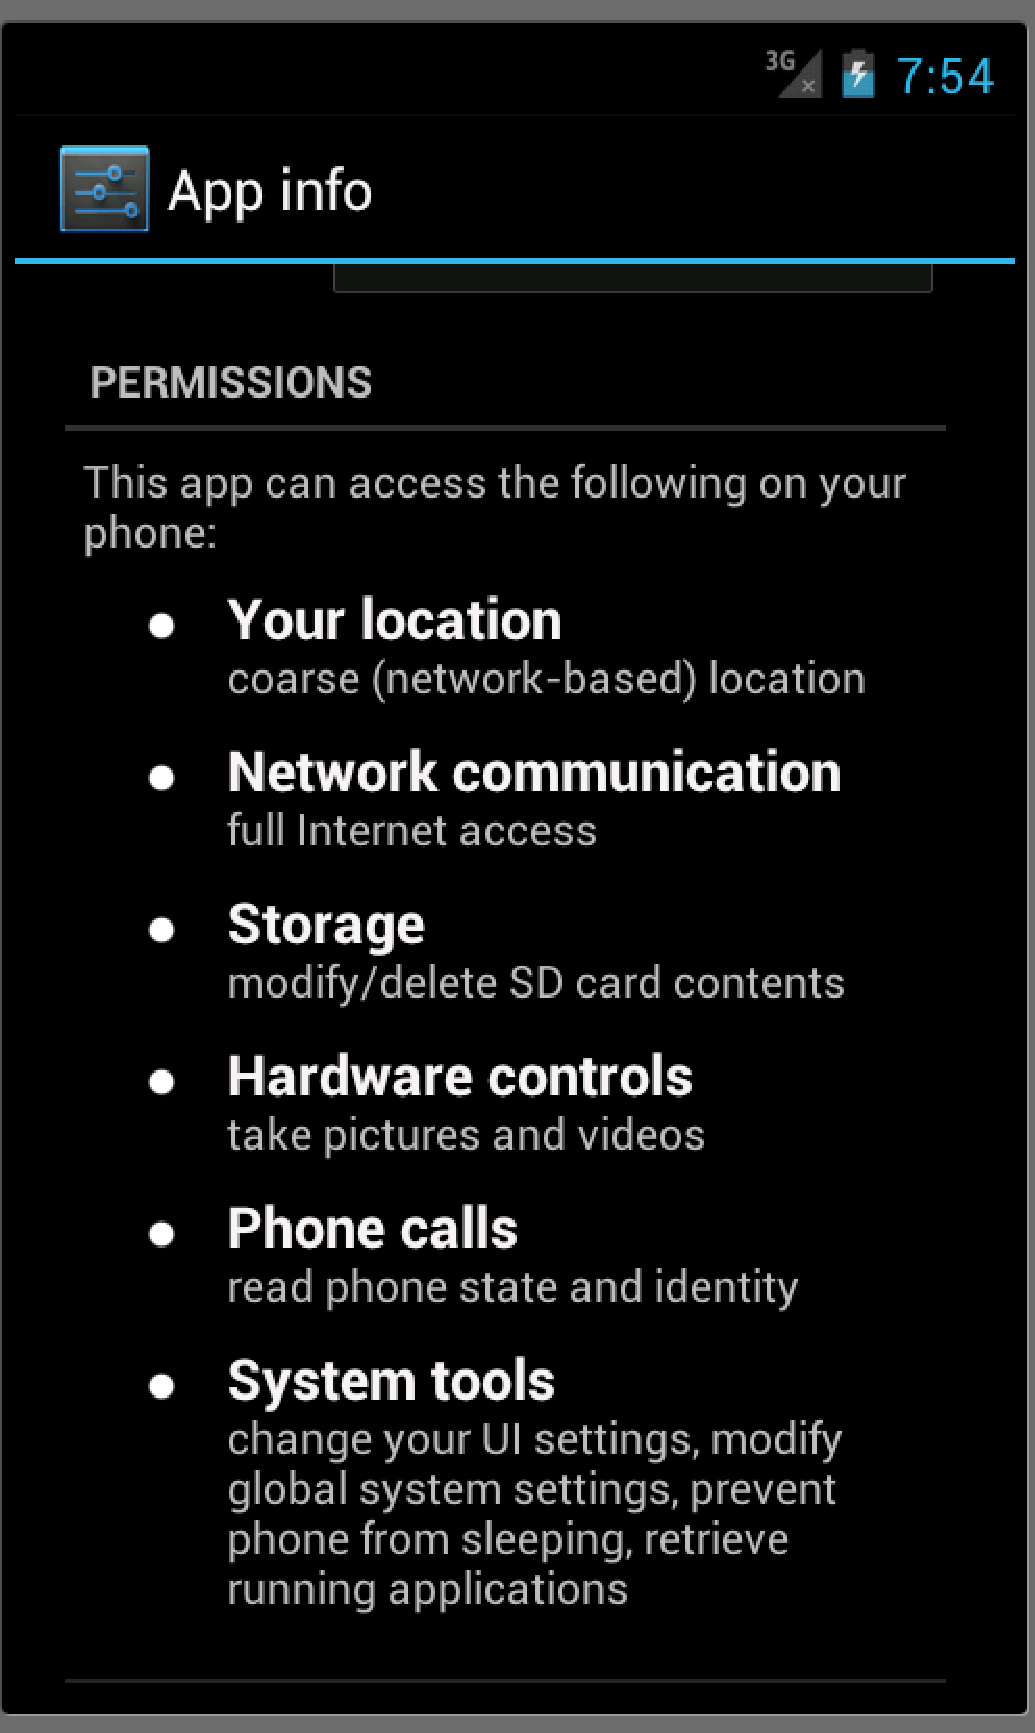
\includegraphics{figure1}}}
\caption{Flashlight app permission requirements}
\label{fig:permission}
\end{figure}

	There are various ways one could remove permissions from Android applications.  Previous work in this area proposes a "privacy mode", where applications running in this mode run with lowered permissions~\cite{Zhou:2011:TISSA}.  This approach requires heavy modification to the Android OS itself, but yields a flexible solution.  Applications can also be repackaged, with their manifests modified to contain fewer permissions.  This is the most popular approach at present, as applications containing this functionality can be readily obtained from major application markets~\cite{Hoffman}.  Additionally, the application's executable code could be dynamically rewritten to protect sensitive API calls~\cite{Davis:2013:RetroSkeleton}.

	All of the above approaches, however, are dependent on Google's policy regarding application permissions, as they influence how developers write their applications. Google's documentation discusses the implementation in enough detail for a developer to use it, but does not go into the rationale behind the approach. While they do suggest that the "dynamic" permission model would be too much of a burden on the user, they do not mention editable static permissions at all. Furthermore, application developers are not explicitly instructed to handle cases of revoked permissions in their applications. Since the lack of a required permission is typically implemented in the form of a Java SecurityException~\cite{Google}, some programmers will handle these gracefully out of habit. However, if an application or library it uses is not explicitly written to handle the permission revocation, modification of the source code will be required to ensure proper function.

\subsection{Effect of Permission Removal}

While previous research has demonstrated that a significant number of Android applications request and use too many permissions~\cite{Felt}, it is unclear how removing permissions would affect the application's behavior.  Under Android's security model, developers typically expect all the requested permissions to be available.  Therefore, it would not be surprising if many developers do not handle the lack of permissions gracefully. When an application invokes an API call without the necessary permissions, it typically throws a \texttt{SecurityException}.  However, if such an exception is caught by library or wrapper code, the application can continue running.  Moreover, permissions are not all equal.  Some permissions describe a devices' hardware capabilities, such as \texttt{CAMERA}.  Since they are not universally available, one would expect libraries to be able to handle their absence more gracefully.  A relatively common instance of this is the removal of the camera on DoD phones for operational security.

When removing a permission, users will expect to see any correlating features be disabled. An everyday example being the removal of GPS capabilities from Google Maps. Currently, many users turn their GPS off in attempts to extend their battery life. When this is done, at launch, the user is notified that the accuracy of Google Maps would be improved if GPS was enabled.  When removing permissions from and application, users are going to expect similar behavior. If an application was not written with permission removal in mind, however, features that are not obviously correlated may malfunction leaving the user confused. This could theoretically include data corruption if the application is not written to handle its data in a robust manner. If this is the case, data would be susceptible to being corrupted if the application crashes regardless of permission removal. While these occurrences are of concern, in the long run, they can easily be addressed by developers.

In this paper, we take the first step to quantitatively measure the effects of removing permissions from Android applications by trying to answer the following questions:

\begin{itemize}
\item How likely will an application crash after a permission is removed?

\item Which permissions, if removed, are less likely to cause an application to crash?

\item Why do applications handle the lack of certain permissions more gracefully?

\end{itemize}

%We chose to test with 7 permissions that we believe have a high potential to result in the compromise of a user's security or privacy.
%While removing a permission may cause many abnormal behaviors, we will focus on crashing, which is likely the most common.  We wish to answer the following questions:
Our work will benefit both users and developers.  Users can make more informed decisions when deciding which permissions to remove (when they use tools for removing permissions).  Application developers can make their code more robust against missing permissions.  Android library developers can design their libraries to handle lack of permissions more gracefully.
	
In the remainder of this paper, we will attempt to quantify the effects of removing permissions from Android applications. In Section \ref{sec:related} we will discuss related work. Then, in Section \ref{sec:method}, we will discuss our methodology and the tool we developed for automated testing, PyAndrazzi. We present the results of our testing in Section \ref{sec:evaluation} and discuss the impact of our findings on users and developers in Section \ref{sec:discussion}. Finally, in Section \ref{sec:future} we discuss future work and conclude with Section \ref{sec:conclusion}. 
